% Options for packages loaded elsewhere
\PassOptionsToPackage{unicode}{hyperref}
\PassOptionsToPackage{hyphens}{url}
\PassOptionsToPackage{dvipsnames,svgnames,x11names}{xcolor}
%
\documentclass[
  11pt,
  ignorenonframetext,
]{beamer}
\usepackage{pgfpages}
\setbeamertemplate{caption}[numbered]
\setbeamertemplate{caption label separator}{: }
\setbeamercolor{caption name}{fg=normal text.fg}
\beamertemplatenavigationsymbolsempty
% Prevent slide breaks in the middle of a paragraph
\widowpenalties 1 10000
\raggedbottom
\setbeamertemplate{part page}{
  \centering
  \begin{beamercolorbox}[sep=16pt,center]{part title}
    \usebeamerfont{part title}\insertpart\par
  \end{beamercolorbox}
}
\setbeamertemplate{section page}{
  \centering
  \begin{beamercolorbox}[sep=12pt,center]{part title}
    \usebeamerfont{section title}\insertsection\par
  \end{beamercolorbox}
}
\setbeamertemplate{subsection page}{
  \centering
  \begin{beamercolorbox}[sep=8pt,center]{part title}
    \usebeamerfont{subsection title}\insertsubsection\par
  \end{beamercolorbox}
}
\AtBeginPart{
  \frame{\partpage}
}
\AtBeginSection{
  \ifbibliography
  \else
    \frame{\sectionpage}
  \fi
}
\AtBeginSubsection{
  \frame{\subsectionpage}
}
\usepackage{amsmath,amssymb}
\usepackage{lmodern}
\usepackage{setspace}
\usepackage{iftex}
\ifPDFTeX
  \usepackage[T1]{fontenc}
  \usepackage[utf8]{inputenc}
  \usepackage{textcomp} % provide euro and other symbols
\else % if luatex or xetex
  \usepackage{unicode-math}
  \defaultfontfeatures{Scale=MatchLowercase}
  \defaultfontfeatures[\rmfamily]{Ligatures=TeX,Scale=1}
\fi
% Use upquote if available, for straight quotes in verbatim environments
\IfFileExists{upquote.sty}{\usepackage{upquote}}{}
\IfFileExists{microtype.sty}{% use microtype if available
  \usepackage[]{microtype}
  \UseMicrotypeSet[protrusion]{basicmath} % disable protrusion for tt fonts
}{}
\makeatletter
\@ifundefined{KOMAClassName}{% if non-KOMA class
  \IfFileExists{parskip.sty}{%
    \usepackage{parskip}
  }{% else
    \setlength{\parindent}{0pt}
    \setlength{\parskip}{6pt plus 2pt minus 1pt}}
}{% if KOMA class
  \KOMAoptions{parskip=half}}
\makeatother
\usepackage{xcolor}
\geometry{left = 1cm, right = 0.5cm, top = 0.5cm, bottom = 0.5cm}
\newif\ifbibliography
\setlength{\emergencystretch}{3em} % prevent overfull lines
\providecommand{\tightlist}{%
  \setlength{\itemsep}{0pt}\setlength{\parskip}{0pt}}
\setcounter{secnumdepth}{-\maxdimen} % remove section numbering
\titlegraphic{
\includegraphics[scale=0.05]{pictures/GlaLogo.pdf}}
\usepackage{float}
\usepackage{booktabs}
\usepackage{array}
\usepackage{longtable}
\setbeamertemplate{itemize item}{$\diamond$}
\setbeamertemplate{itemize subitem}{\scriptsize$\diamond$}
\setbeamertemplate{itemize subsubitem}{\scriptsize$\gg$}
\ifLuaTeX
  \usepackage{selnolig}  % disable illegal ligatures
\fi
\IfFileExists{bookmark.sty}{\usepackage{bookmark}}{\usepackage{hyperref}}
\IfFileExists{xurl.sty}{\usepackage{xurl}}{} % add URL line breaks if available
\urlstyle{same} % disable monospaced font for URLs
\hypersetup{
  pdftitle={Introductory Statistics for Economics},
  pdfauthor={Duong Trinh},
  colorlinks=true,
  linkcolor={blue},
  filecolor={Maroon},
  citecolor={Blue},
  urlcolor={Blue},
  pdfcreator={LaTeX via pandoc}}

\title{Introductory Statistics for Economics}
\subtitle{ECON1013: TUTORIAL 1}
\author{Duong Trinh}
\date{2025}
\institute{University of Glasgow}

\begin{document}
\frame{\titlepage}

\setstretch{1.5}
\begin{frame}{Intro}
\protect\hypertarget{intro}{}
\begin{itemize}
\tightlist
\item
  Duong Trinh

  \begin{itemize}
  \tightlist
  \item
    PhD Student in Economics (Bayesian Microeconometrics)
  \item
    Email: \underline{Duong.Trinh@glasgow.ac.uk}
  \end{itemize}
\end{itemize}

\vspace{3mm}

\begin{itemize}
\tightlist
\item
  ECON1013 TU07

  \begin{itemize}
  \tightlist
  \item
    Tuesday 2-3 pm
  \item
    4 sessions (28-Jan, 11-Feb, 25-Feb, 11-March)
  \end{itemize}
\item
  ECON1013-TU08

  \begin{itemize}
  \tightlist
  \item
    Tuesday 3-4 pm
  \item
    4 sessions (28-Jan, 11-Feb, 25-Feb, 11-March)
  \end{itemize}
\end{itemize}
\end{frame}

\begin{frame}{Record Attendance}
\protect\hypertarget{record-attendance}{}
\end{frame}

\begin{frame}{Exercise 1}
\protect\hypertarget{exercise-1}{}
A group of \(11\) former college students are interviewed \(10\) years
after their graduation. Their incomes are as follows (in \(1,000\)
pounds): \[
\{20, 22, 23, 23, 25, 28, 28, 30, 30, 34, 160\}
\] For this sample, we have calculated the following summary statistics:

\begin{itemize}
\item
  Sample average \(\approx 38.5\)
\item
  Sample median \(28\)
\item
  Sample standard deviation \(40.5\)
\item
  Interquartile range \(7\) (from \(23\) to \(30\))
\end{itemize}
\end{frame}

\begin{frame}{Exercise 1}
\protect\hypertarget{exercise-1-1}{}
A group of \(11\) former college students are interviewed \(10\) years
after their graduation. Their incomes are as follows (in \(1,000\)
pounds): \[
\{20, 22, 23, 23, 25, 28, 28, 30, 30, 34, 160\}
\]

\begin{enumerate}
[a.]
\item
  We wish to measure the central tendency in this sample. Which measure
  is the most appropriate? (You can use the summary statistics provided
  above or other measures.) Argue.
\item
  We wish to measure the variability in this sample. Which measure is
  the most appropriate? (You can use the summary statistics provided
  above or other measures.) Argue.
\item
  Construct a box-and-whisker plot of the data.
\item
  There was a reporting mistake in the data set - the largest value is
  actually \(360\) instead of \(160\). How do the summary statistics
  change? Do your answers to questions 1 and 2 change?
\end{enumerate}
\end{frame}

\begin{frame}[fragile]{(a) We wish to measure the central tendency in
this sample. Which measure is the most appropriate?}
\protect\hypertarget{a-we-wish-to-measure-the-central-tendency-in-this-sample.-which-measure-is-the-most-appropriate}{}
\pause

\begin{verbatim}
## Warning: package 'knitr' was built under R version 4.2.3
\end{verbatim}

\begin{center}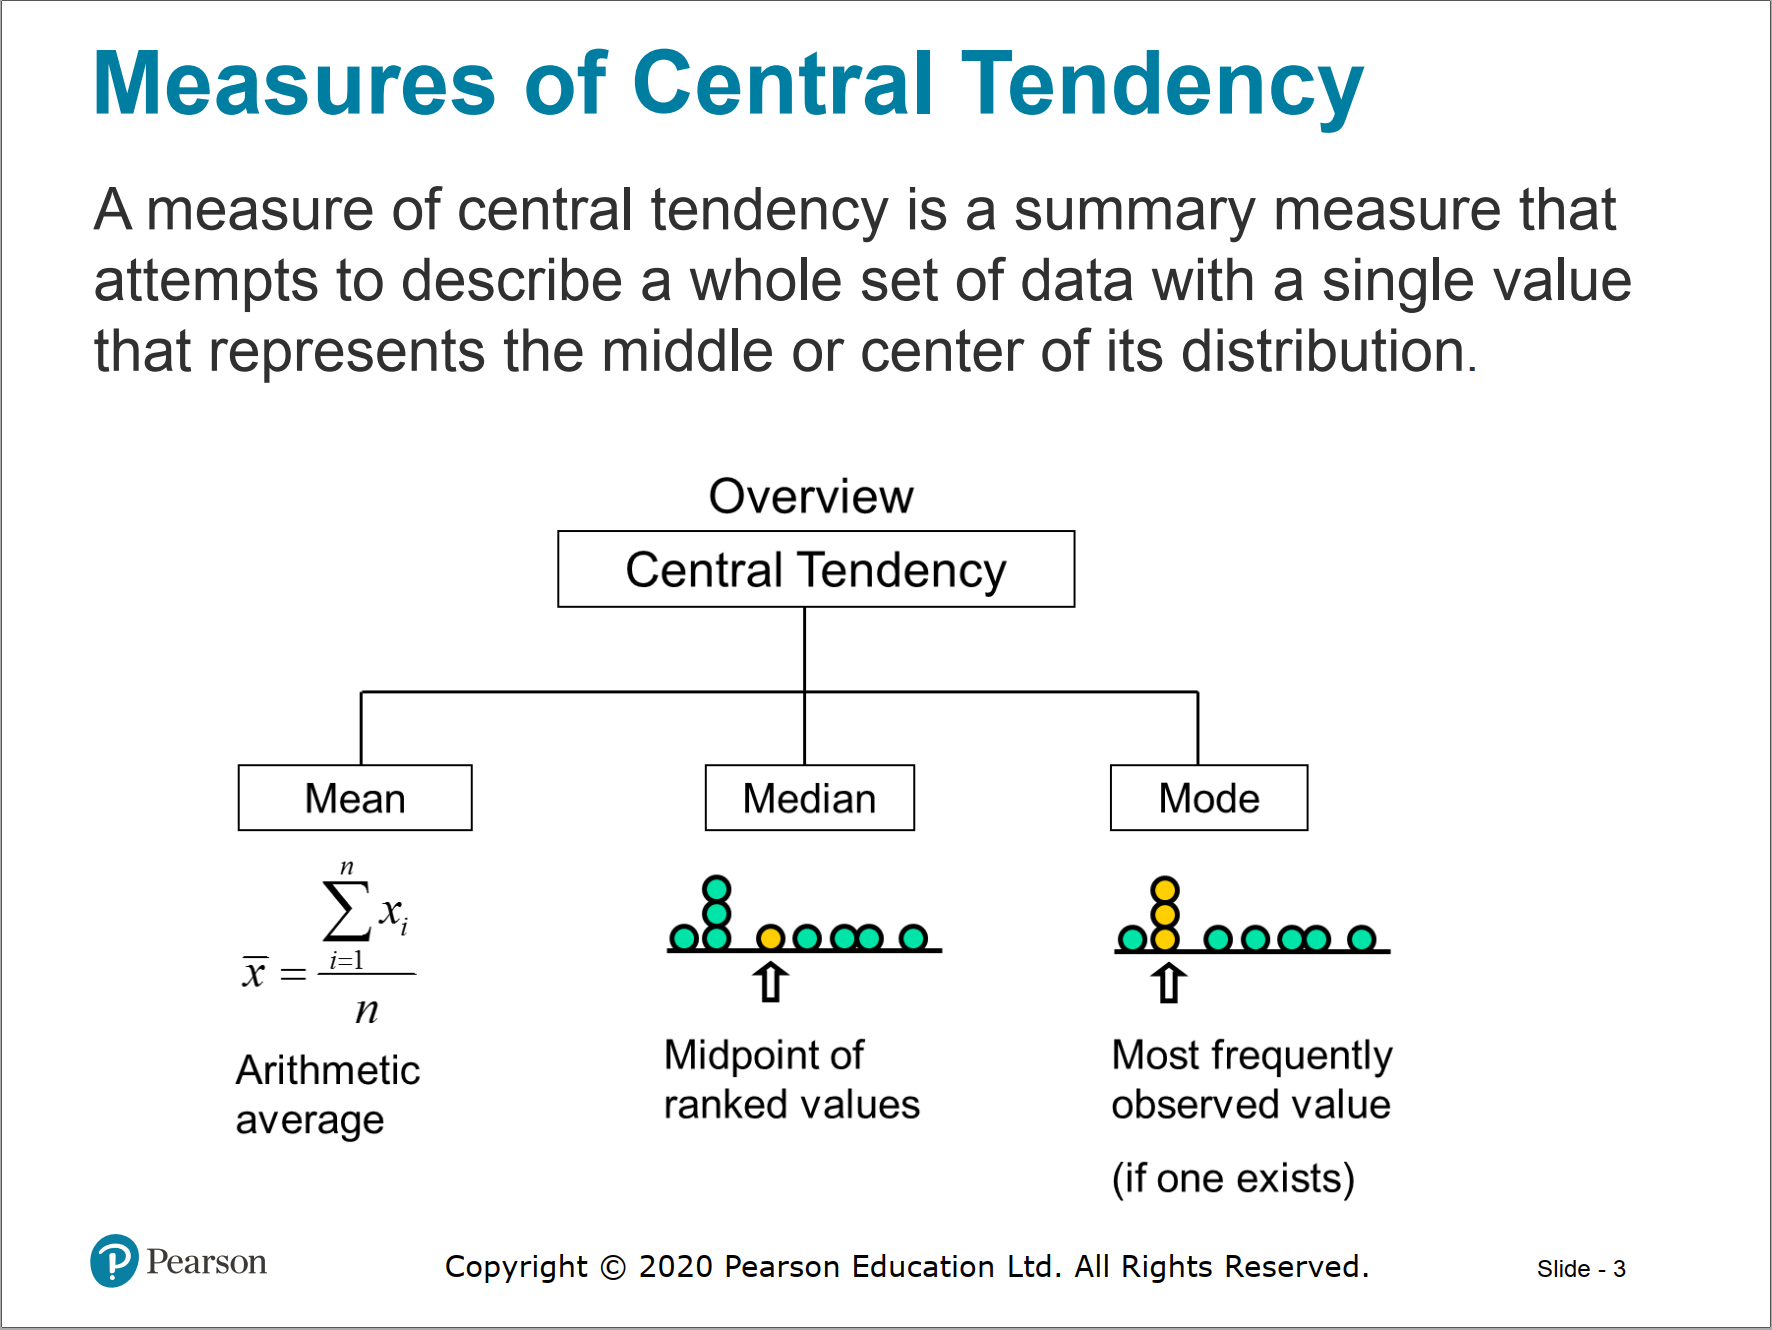
\includegraphics[width=0.8\linewidth]{pictures/Central Tendency} \end{center}
\end{frame}

\begin{frame}{(a) We wish to measure the central tendency in this
sample. Which measure is the most appropriate?}
\protect\hypertarget{a-we-wish-to-measure-the-central-tendency-in-this-sample.-which-measure-is-the-most-appropriate-1}{}
\begin{itemize}
\item
  The distribution is characterised by a cluster of observations around
  \(30\) and a single large outlier.
\item
  Because of this outlier, sample mean is significantly larger than the
  values in the main cluster of observations.
\item
  Sample median gives a more accurate description of the main cluster of
  observations.
\end{itemize}
\end{frame}

\begin{frame}{(b) We wish to measure the variability in this sample.
\quad Which measure is the most appropriate?}
\protect\hypertarget{b-we-wish-to-measure-the-variability-in-this-sample.-which-measure-is-the-most-appropriate}{}
\pause

\begin{center}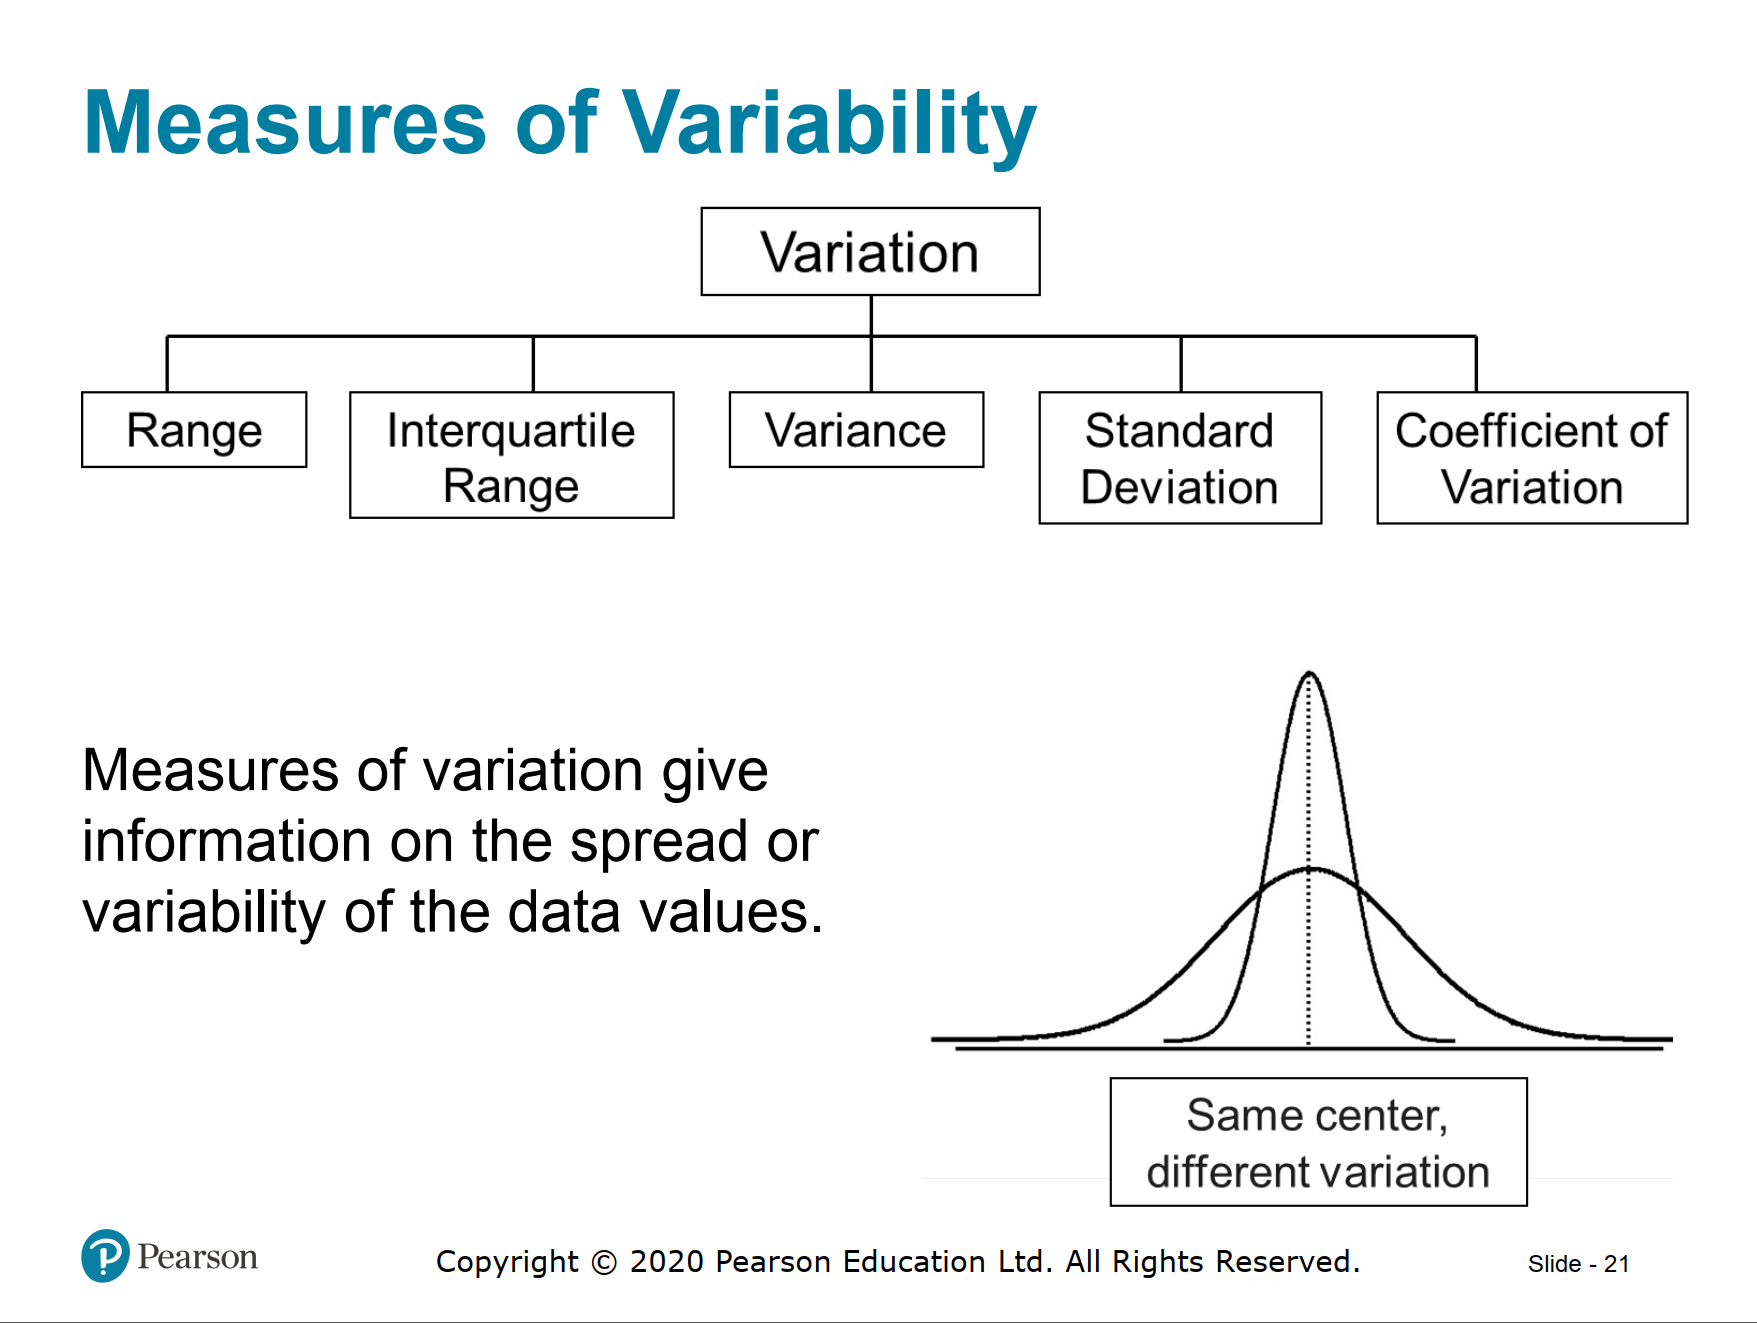
\includegraphics[width=0.8\linewidth]{pictures/Variability} \end{center}
\end{frame}

\begin{frame}{(b) We wish to measure the variability in this sample.
\quad Which measure is the most appropriate?}
\protect\hypertarget{b-we-wish-to-measure-the-variability-in-this-sample.-which-measure-is-the-most-appropriate-1}{}
\begin{itemize}
\item
  The sample standard deviation depends on the sample mean. Since the
  sample mean is affected by the single outlier, so is the sample
  standard deviation. As a consequence, the sample standard deviation is
  high, which indicates a high degree of variability in the data.
\item
  However, in the main cluster of observations, values are relatively
  close to each other.
\item
  This is more informatively summarized by the interquartile range
  (\(7\)), which indicates a relatively low degree of variability in the
  data.
\end{itemize}
\end{frame}

\begin{frame}{(c) Construct a box-and-whisker plot of the data.}
\protect\hypertarget{c-construct-a-box-and-whisker-plot-of-the-data.}{}
\pause

\begin{itemize}
\tightlist
\item
  The box-and-whisker plot usually displays \(5\) values:\\
  The minimum, the \(25^{th}\) percentile, the median, the \(75^{th}\)
  percentile, and the maximum.
\end{itemize}

\begin{center}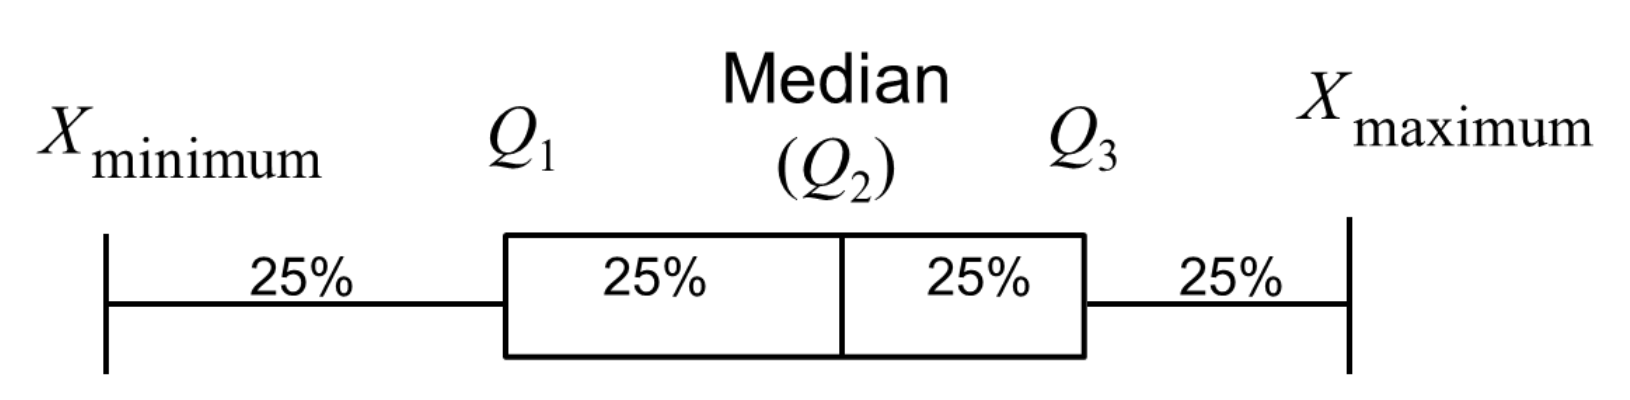
\includegraphics[width=0.7\linewidth]{pictures/Box-and-Whisker} \end{center}
\end{frame}

\begin{frame}{(d) There was a reporting mistake in the data set - the
largest value is actually \(360\) instead of \(160\). How do the summary
statistics change? Do your answers to questions 1 and 2 change?}
\protect\hypertarget{d-there-was-a-reporting-mistake-in-the-data-set---the-largest-value-is-actually-360-instead-of-160.-how-do-the-summary-statistics-change-do-your-answers-to-questions-1-and-2-change}{}
\pause

Our summary statistics change as follows:

\begin{itemize}
\item
  Sample average \(\approx 56.6\)
\item
  Sample median \(28\)
\item
  Sample standard deviation \(100.7\)
\item
  Interquartile range \(7\) (from \(23\) to \(30\))
\end{itemize}

Sample median and interquartile range are not affected by the value of
the outlier.
\end{frame}

\begin{frame}{Exercise 2}
\protect\hypertarget{exercise-2}{}
Consider the sample \(\{X_1, X_2, \ldots, X_n\}\).

\begin{enumerate}
[a.]
\item
  Show that \(\bar{X}_n = \frac{1}{n} \sum_{i=1}^n X_i\) is the solution
  of minimization problem: \[
  \tag{1}
  \underset{c}{\text{min}} \sum_{i=1}^{n} \left(X_i - c\right)^2
  \]
\item
  What is the interpretation of the function
  \(\sum_{i=1}^{n} \left(X_i - c\right)^2\)?
\end{enumerate}

\emph{(The aim of this exercise is justify the use of the sample
average).}
\end{frame}

\begin{frame}{(a) Show that \(\bar{X}_n = \frac{1}{n} \sum_{i=1}^n X_i\)
is the solution of \quad  minimization problem \((1)\)}
\protect\hypertarget{a-show-that-barx_n-frac1n-sum_i1n-x_i-is-the-solution-of-minimization-problem-1}{}
\pause

\begin{itemize}
\tightlist
\item
  Let
  \(h(c) = \sum_{i=1}^{n} \left(X_i - c\right)^2 = \sum_{i=1}^{n}\left(X_i^2 - 2 X_i c + c^2\right)\)
\end{itemize}

\pause

\begin{itemize}
\tightlist
\item
  To find the minimum, we take the first-order condition w.r.t. \(c\):
  \[
  h'(c) = \sum_{i=1}^{n} \left(-2 X_i + 2 c\right) = -2\sum_{i=1}^n \left(X_i-c\right)
  \]
\end{itemize}

\pause

\begin{itemize}
\tightlist
\item
  We wish to solve for \(c\) such that \(h'(c) = 0\): \[
  \begin{aligned}
  h'(c) = 0 &\Leftrightarrow \sum_{i=1}^n \left(X_i-c\right) = 0\\
  &\Leftrightarrow \left(X_1-c\right) + \left(X_2-c\right) + \ldots + \left(X_n-c\right) = 0\\
  &\Leftrightarrow -nc + \sum_{i=1}^{n} X_i = 0\\
  &\Leftrightarrow c = \frac{1}{n} \sum_{i=1}^n X_i
  \end{aligned}
  \] which is what we wanted to show.
\end{itemize}
\end{frame}

\begin{frame}{(b) What is the interpretation of the function
\(\sum_{i=1}^{n} \left(X_i - c\right)^2\)?}
\protect\hypertarget{b-what-is-the-interpretation-of-the-function-sum_i1n-leftx_i---cright2}{}
\begin{itemize}
\item
  The term \(X_i-c\) is the difference between each observation and some
  constant \(c\). These differences are sometimes positive and sometimes
  negative - but if we square them, they are always positive.
\item
  The summation \(\sum_{i=1}^n \left(X_i-c\right)\) gives us the sum of
  squared differences. When we solve the minimization, we are looking
  for the value of c such that the sum of squared differences between
  each observation and \(c\) is the smallest possible.
\item
  In other words, we are looking for \(c\) such that \(c\) is closest
  possible to different values of \(X_i\), when ``closest possible'' is
  measured by the squared differences.
\item
  Thus, the sample mean is the quantity which minimizes the sum of
  squared differences in the data.
\end{itemize}
\end{frame}

\begin{frame}{(b) What is the interpretation of the function
\(\sum_{i=1}^{n} \left(X_i - c\right)^2\)?}
\protect\hypertarget{b-what-is-the-interpretation-of-the-function-sum_i1n-leftx_i---cright2-1}{}
\textbf{Remark.} Notice that the sample median is the solution of the
problem: \[
\tag{2}
\underset{c}{\text{min}} \sum_{i=1}^{n} \mid X_i - c\mid
\]

\begin{itemize}
\tightlist
\item
  Thus, while sample mean minimizes sum of squared differences, sample
  median minimizes the sum of absolute differences.
\item
  The ``best'' measure of central tendency depends on the measure of
  distance that we want to minimize.
\end{itemize}
\end{frame}

\begin{frame}{Exercise 3}
\protect\hypertarget{exercise-3}{}
\begin{enumerate}
[a.]
\tightlist
\item
  Show that
  \(\sum_{i=1}^n \left(X_i - \bar{X}_n\right)^2 = \sum_{i=1}^n X_i^2 - n \bar{X}_n^2\).\\
  What is this estimator?
\end{enumerate}

\vspace{3mm}

\begin{enumerate}
[a.]
\setcounter{enumi}{1}
\tightlist
\item
  Show that
  \(\sum_{i=1}^n \left(X_i - \bar{X}_n\right)\left(Y_i - \bar{Y}_n\right) = \sum_{i=1}^n \left(X_i - \bar{X}_n\right)Y_i = \sum_{i=1}^n X_i Y_i - n\bar{X}_n\bar{Y}_n\).\\
  What is this estimator?
\end{enumerate}
\end{frame}

\begin{frame}{(a) Show that
\(\sum_{i=1}^n \left(X_i - \bar{X}_n\right)^2 = \sum_{i=1}^n X_i^2 - n \bar{X}_n^2\).}
\protect\hypertarget{a-show-that-sum_i1n-leftx_i---barx_nright2-sum_i1n-x_i2---n-barx_n2.}{}
\pause

We are showing a property related to \emph{sample variance}.

\pause

\[
\begin{aligned}
\sum_{i=1}^n \left(X_i - \bar{X}_n\right)^2  &= \sum_{i=1}^n \left(X_i^2 - 2X_i\bar{X}_n + \bar{X}_n^2\right)\\
&= \sum_{i=1}^n X_i^2  - 2 \bar{X}_n \sum_{i=1}^n X_i + n \bar{X}_n^2\\
&= \sum_{i=1}^n X_i^2  - 2 \bar{X}_n \cdot n \bar{X}_n + n \bar{X}_n^2\\
&= \sum_{i=1}^n X_i^2  - 2n \bar{X}_n^2 + n \bar{X}_n^2\\
&= \sum_{i=1}^n X_i^2 - n \bar{X}_n^2
\end{aligned}
\] proving the result.
\end{frame}

\begin{frame}{(b) Show that
\(\sum_{i=1}^n \left(X_i - \bar{X}_n\right)\left(Y_i - \bar{Y}_n\right) = \sum_{i=1}^n \left(X_i - \bar{X}_n\right)Y_i = \sum_{i=1}^n X_i Y_i - n\bar{X}_n\bar{Y}_n\).}
\protect\hypertarget{b-show-that-sum_i1n-leftx_i---barx_nrightlefty_i---bary_nright-sum_i1n-leftx_i---barx_nrighty_i-sum_i1n-x_i-y_i---nbarx_nbary_n.}{}
\pause

We are showing a property related to \emph{sample covariance}.

\pause

\[
\begin{aligned}
\sum_{i=1}^n \left(X_i - \bar{X}_n\right)\left(Y_i - \bar{Y}_n\right) &= \sum_{i=1}^n \left(X_i - \bar{X}_n\right)Y_i - \sum_{i=1}^n \left(X_i - \bar{X}_n\right)\bar{Y}_n\\
&= \sum_{i=1}^n \left(X_i - \bar{X}_n\right)Y_i\\
\end{aligned}
\]\\
because
\(\sum_{i=1}^n\left(X_i - \bar{X}_n\right) = \sum_{i=1}^n X_i - n\bar{X}_n = 0\).

It follows that \[ 
\sum_{i=1}^n \left(X_i - \bar{X}_n\right)Y_i = \sum_{i=1}^n X_iY_i - \bar{X}_n\sum_{i=1}^nY_i = \sum_{i=1}^n X_iY_i - n\bar{X}_n\bar{Y}_n.
\]
\end{frame}

\end{document}
